\documentclass[a4paper,11pt]{article}

\usepackage{préambule}

\newgeometry{top=1cm,bottom=1cm,left=1cm,right=1cm}

\makeatletter
\renewcommand{\maketitle}{%
{\scriptsize colle dans ton cahier d'exercices}
	\begin{center}
		\LARGE
		\myuline{\@title}
		\vspace{1em}
	\end{center}
}
\makeatother

\title{Dessiner avec scratch}
\author{}
\date{}

\begin{document}

\maketitle

On va faire des dessins en utilisant Scratch.

\section{Mise en place}

\begin{enumerate}[1)]
	\item Démarre Scratch, et commence un nouveau projet.
	\item Pour accéder au stylo, appuie sur le bouton d'extensions : 
\includegraphics[height=1.5em]{Images/Scratch 3 - bouton extensions.png}, et clique sur « stylo ».

	      Il y a maintenant un nouveau type de blocks : 
\includegraphics[height=2em]{Images/Scratch 3 - block stylos.png}.
	\item Ensuite, suis les instructions suivantes :
	      \begin{itemize}
		      \item Clique sur « Mes blocks », puis sur « Créer un block ».
		      \item Nomme ce block « Efface tout », et appuie sur « OK ».
		      \item Accroche les instructions suivantes au nouveau block :
		            \begin{itemize}
			            \item[] \squared[Orchid]{cacher}
			            \item[] \squared[Cyan]{mettre x à \circled{0}}
			            \item[] \squared[Cyan]{mettre y à \circled{0}}
			            \item[] \squared[Cyan]{s'orienter en direction de \circled{90}}
			            \item[] \squared[TealBlue]{
\includegraphics[height=1.5em]{Images/Scratch 3 - stylo icon.png} stylo en position d'écriture}
			            \item[] \squared[TealBlue]{
\includegraphics[height=1.5em]{Images/Scratch 3 - stylo icon.png} effacer tout}
		            \end{itemize}
	      \end{itemize}
	      Tu peux maintenant utiliser le block \squared[Salmon]{Efface tout} pour effacer le dessin et mettre le stylo au centre de l'écran.
\end{enumerate}

\section{Premiers dessins}

\begin{enumerate}
	\item Utilise à la suite le block \squared[Salmon]{Efface tout} et \squared[Cyan]{avance \circled{50}}.

	      La ligne obtenue est-elle \vspace{0.5em}

	      \hspace{3em} verticale \hfill horizontale \hspace{3em}

	      ?
	\item  Au début du programme, les coordonnées du stylo sont (0 ; 0). Après ce programme, quelles sont les coordonnées du stylo ? ................
	\item Utilise les block \squared[Cyan]{avance \circled{\phantom{A}}} et \squared[Cyan]{tourner de \circled{\phantom{A}}} pour dessiner un carré.
\end{enumerate}

\section{Dessins complexes}

Utilise le stylo pour faire les dessins suivants : 

\hfill → {\footnotesize Tourne la page}

\begin{enumerate}[1)]
	\item \begin{center}
		      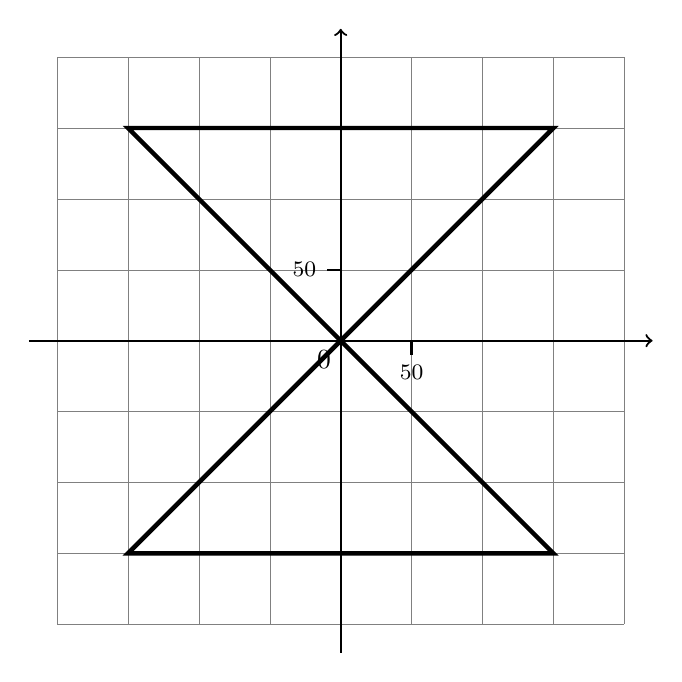
\begin{tikzpicture}[scale=0.018]
			      \draw[gray,ultra thin,step=50] (-200,-200) grid (200,200);
			      \draw[thick,->] (-220,0) -- (220,0);
			      \draw[thick,->] (0,-220) -- (0,220);

			      \draw[thick] (50,0) -- (50,-10) node[below] {\footnotesize 50};
			      \draw[thick] (0,50) -- (-10,50) node[left] {\footnotesize 50};
			      \node[below left] at (0,0) {0};

			      \draw[ultra thick] (0,0) -- ++(150,150) -- ++(-300,0) -- ++(300,-300) -- ++(-300,0) -- cycle;
		      \end{tikzpicture}
	      \end{center}
	\item \begin{center}
		      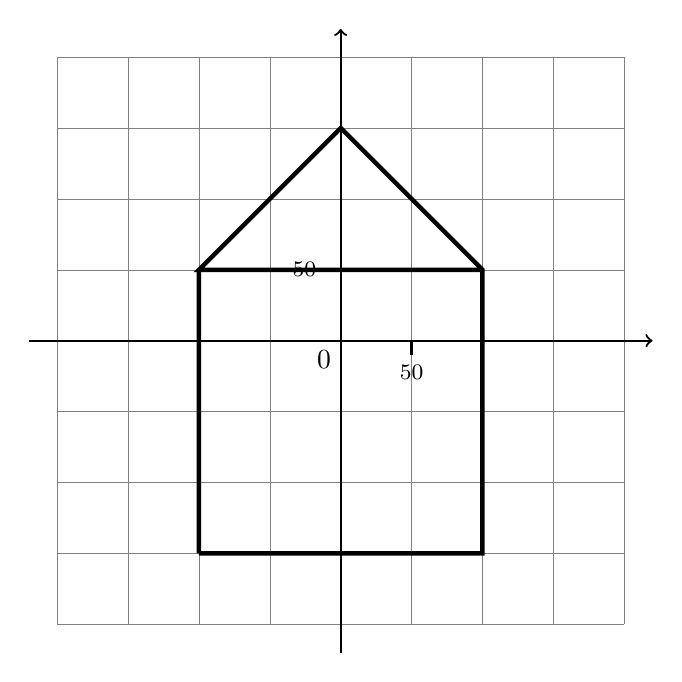
\begin{tikzpicture}[scale=0.018]
			      \draw[gray,ultra thin,step=50] (-200,-200) grid (200,200);
			      \draw[thick,->] (-220,0) -- (220,0);
			      \draw[thick,->] (0,-220) -- (0,220);

			      \draw[thick] (50,0) -- (50,-10) node[below] {\footnotesize 50};
			      \draw[thick] (0,50) -- (-10,50) node[left] {\footnotesize 50};
			      \node[below left] at (0,0) {0};

			      \draw[ultra thick] (-100,-150) -- ++(200,0) -- ++(0,200) -- ++(-100,100) -- ++(-100,-100) -- ++(200,0) ++(-200,0) -- ++(0,-200);
		      \end{tikzpicture}
	      \end{center}
	\item \begin{center}
		      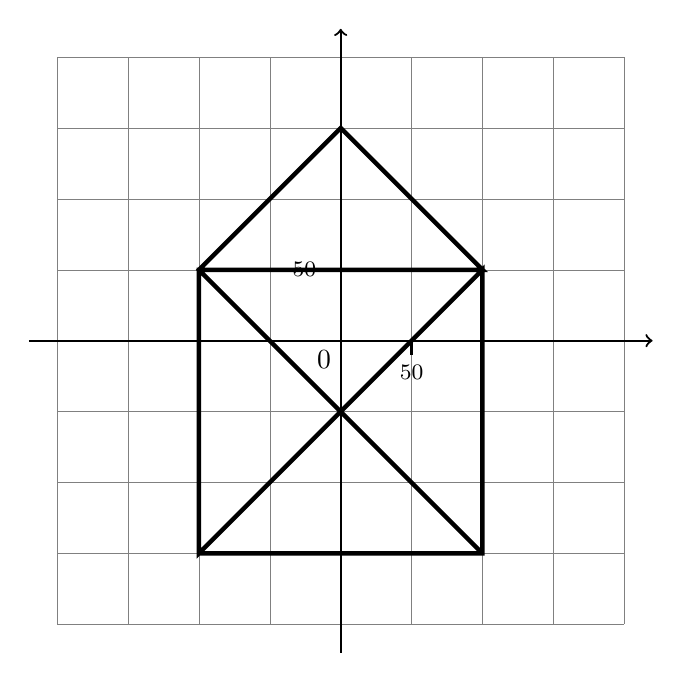
\begin{tikzpicture}[scale=0.018]
			      \draw[gray,ultra thin,step=50] (-200,-200) grid (200,200);
			      \draw[thick,->] (-220,0) -- (220,0);
			      \draw[thick,->] (0,-220) -- (0,220);

			      \draw[thick] (50,0) -- (50,-10) node[below] {\footnotesize 50};
			      \draw[thick] (0,50) -- (-10,50) node[left] {\footnotesize 50};
			      \node[below left] at (0,0) {0};

			      \draw[ultra thick] (-100,-150) -- ++(200,0) -- ++(0,200) -- ++(-200,-200) -- ++(0,200) -- ++(200,0) -- ++(-100,100) -- ++(-100,-100) -- ++(200,-200);
		      \end{tikzpicture}
	      \end{center}

	\item Pour visualiser les mouvements du stylo, on peut utiliser le block

	      \squared[Cyan]{glisser en \circled{\phantom{A}} secondes à x: \circled{\phantom{A}} y: \circled{\phantom{A}}}

	      Peux-tu reproduire le dessin de la question 3) sans que le stylo repasse sur la même ligne deux fois ?

	      Peux-tu le faire sans utiliser \squared[TealBlue]{
\includegraphics[height=1.5em]{Images/Scratch 3 - stylo icon.png} relever le stylo} ?
\end{enumerate}

\end{document}